\section{Modelando problemas de controladores dinámicamente actualizables}

Agregamos un conjunto de palabras reservadas a FSP para poder soportar objetivos actualizables. En la figura
\ref{MTSA_example} mostramos el código FSP necesario para síntesis de controladores actualizables para el ejemplo del reactor nuclear
presentado en la sección \ref{power_plant}.

El operador \texttt{\textbf{updatingController}} es utilizado para definir el problema de controladores
actualizables. Al ejecutar la composición en paralelo de este elemento obtendremos, si existe, un controlador que satisface los
objetivos del problema de control sin violar la especificación del ambiente de actualización. Ambos definidos en el
capítulo \ref{updating_controller_chapter}. Necesitamos en esta declaración, además de los nuevos requerimientos, suministrar
el controlador actual, el modelo del ambiente actual, el modelo del ambiente nuevo y un conjunto de pares de flujos
donde cada elemento indicará correspondencia de propiedades del ambiente actual al ambiente nuevo como dijimos en la
definición \ref{update_environment_def}. Por ejemplo, en la figura \ref{MTSA_example} podemos observar que al usar la
palabra reservada \texttt{\textbf{updatingController}} configuramos \textsc{EnvironmentAndController} como el
controlador actual, \textsc{OldEnvironment} como modelo del ambiente actual, \textsc{NewEnvironment} como modelo del
ambiente nuevo, \texttt{\textbf{UpdateSpec}} como la nueva especificación y \textsc{\{\{RequestPending,RequestPending\},
\{IsStopped,IsStopped\}\}} es el conjunto de flujos. Para este ejemplo, \textsc{OldEnvironment} y
\textsc{NewEnvironment} poseen distintos nombres, pero son el mismo ambiente puesto a que este ejemplo es una
actualización que no requiere hacer un cambio en el ambiente.

Los objetivos nuevos están definidos mediante el operador \texttt{\textbf{controllerSpec}}. La palabra reservada
\texttt{\textbf{safety}} permite definir requerimientos de seguridad (\emph{safety}). Aquí incluiremos fórmulas
LTL definidas en la sección \ref{LTL} . La sección de \emph{liveness} esta definida usando los operadores \texttt{\textbf{assumption}} y
\texttt{\textbf{liveness}} que especifican las asunciones del ambiente y objetivos de \emph{liveness} respectivamente.
Ambas deberán definirse mediante FLTLs. En el ejemplo EL EJEMPLO. Luego, el controlador sintetizado nos garantizará que
si infinitamente la actualización es requerida (i.e sucede la acción $beginUpdate$), las acciones $stopOldSpec$ y
$startNewSpec$ sucederán infinitamente. Por último la sección de \texttt{\textbf{controllableActions}} detalla el
conjunto de acciones consideradas controlables a la hora de resolver el problema de control.


\begin{figure}
    \centering
    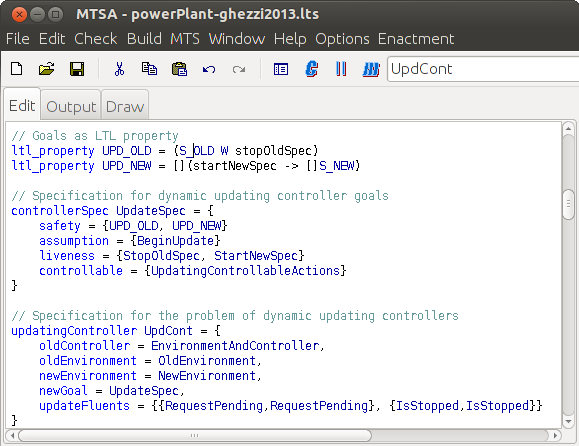
\includegraphics[scale=0.5]{img/MTSA_example.png}
    \caption{MTSA -- Definición de problema de controladores dinámicamente actualizables}
    \label{MTSA_example}
\end{figure}

